%%%%%%%%%%%%%%%%%%%%%%%%%%%%%%%%%%%%%%%%%
% Poster for the PaPE Conference 2017 by Bradley Rentz and Victoria Anderson
% Code adapted from:
% baposter Landscape Poster
% LaTeX Template
% Version 1.0 (11/06/13)
%
% baposter Class Created by:
% Brian Amberg (baposter@brian-amberg.de)
%
% This template has been downloaded from:
% http://www.LaTeXTemplates.com
%
% License:
% CC BY-NC-SA 3.0 (http://creativecommons.org/licenses/by-nc-sa/3.0/)
%
%%%%%%%%%%%%%%%%%%%%%%%%%%%%%%%%%%%%%%%%%

%----------------------------------------------------------------------------------------
%	PACKAGES AND OTHER DOCUMENT CONFIGURATIONS
%----------------------------------------------------------------------------------------

% Note: to compile need fonts: Source Sans Pro & Univers LT Std

\documentclass[portrait,fontscale=0.285,a0paper]{baposter2}
 % Adjust the font scale/size here
 


\usepackage{graphicx} % Required for including images
\graphicspath{{figures/}} % Directory in which figures are stored

\usepackage{amsmath} % For typesetting math
\usepackage{amssymb} % Adds new symbols to be used in math mode

\usepackage{booktabs} % Top and bottom rules for tables
\usepackage{enumitem} % Used to reduce itemize/enumerate spacing
%\usepackage{palatino} % Use the Palatino font
\usepackage[font=small,labelfont=bf]{caption} % Required for specifying captions to tables and figures

\usepackage{multicol} % Required for multiple columns
\setlength{\columnsep}{1.5em} % Slightly increase the space between columns
\setlength{\columnseprule}{0mm} % No horizontal rule between columns

\usepackage{subcaption}
\usepackage{setspace}

\usepackage{tikz} % Required for flow chart
\usetikzlibrary{shapes,arrows} % Tikz libraries required for the flow chart in the template

\newcommand{\compresslist}{ % Define a command to reduce spacing within itemize/enumerate environments, this is used right after \begin{itemize} or \begin{enumerate}
\setlength{\itemsep}{1pt}
\setlength{\parskip}{0pt}
\setlength{\parsep}{0pt}
}
\usepackage{natbib}
\bibpunct[: ]{(}{)}{,}{a}{}{,}
	\newcommand{\BIBand}{\&}
	\setlength{\bibsep}{0pt}
	\setlength{\bibhang}{0.25in}
	\bibliographystyle{sp}



\usepackage{fontspec}
\newcommand{\timesm}{\fontspec[
Contextuals={Inner,WordFinal,WordInitial},Ligatures={Common,TeX},Numbers={OldStyle}]{Sabon LT Std}\fontsize{10pt}{13.5pt}\selectfont}%

\newcommand{\sansipa}{\fontspec[
Contextuals={Inner,WordFinal,WordInitial},Ligatures={Common,TeX},Numbers={OldStyle}]{Source Sans Pro Light}\fontsize{15pt}{13.5pt}\selectfont}%

\usepackage[activate={true,nocompatibility},
  final,
%  tracking=true, % breaks sc
  factor=1200,
  stretch=50,
  shrink=0
  ]{microtype}

\pdfprotrudechars=2
\pdfadjustspacing=2
\newfontfeature{Microtype}{protrusion=default;expansion=default}
\directlua{fonts.protrusions.setups.default.factor=.5}
\defaultfontfeatures{Mapping=text-text}

\setmainfont[BoldFont={Univers LT Std Bold},Contextuals={Inner,WordFinal,WordInitial},ItalicFont={UniversLTStd-LightObl},Ligatures={Common,TeX}]{Univers LT Std Light}\fontsize{9.5pt}{10.5pt}

\newcommand{\ipa}{\fontspec[
Contextuals={Inner,WordFinal,WordInitial},Ligatures={Common,TeX},Numbers={OldStyle}]{Source Sans Pro Light}\fontsize{9.5pt}{10.5pt}\selectfont}

\newcommand{\mainfont}{\fontspec[BoldFont={Univers LT Std Bold},
Contextuals={Inner,WordFinal,WordInitial},Ligatures={Common,TeX},ItalicFont={UniversLTStd-LightObl},Numbers={OldStyle}]{Univers LT Std Light}\fontsize{9.5pt}{10.5pt}\selectfont}


\definecolor{lightblue}{RGB}{2,71,49} % Defines the color used for content box headers

\begin{document}
\mainfont
\begin{poster}
{
headerborder=closed, % Adds a border around the header of content boxes
colspacing=1em, % Column spacing
bgColorOne=white, % Background color for the gradient on the left side of the poster
bgColorTwo=white, % Background color for the gradient on the right side of the poster
borderColor=lightblue, % Border color
headerColorOne=darkgray, % Background color for the header in the content boxes (left side)
headerColorTwo=lightblue, % Background color for the header in the content boxes (right side)
headerFontColor=white, % Text color for the header text in the content boxes
boxColorOne=white, % Background color of the content boxes
textborder=roundedleft, % Format of the border around content boxes, can be: none, bars, coils, triangles, rectangle, rounded, roundedsmall, roundedright or faded
eyecatcher=true, % Set to false for ignoring the left logo in the title and move the title left
headerheight=0.1\textheight, % Height of the header
headershape=roundedright, % Specify the rounded corner in the content box headers, can be: rectangle, small-rounded, roundedright, roundedleft or rounded
headerfont=\mainfont\Large\bf, % Large, bold and sans serif font in the headers of content boxes
%textfont={\setlength{\parindent}{1.5em}}, % Uncomment for paragraph indentation
linewidth=2pt % Width of the border lines around content boxes
}
%----------------------------------------------------------------------------------------
%	TITLE SECTION 
%----------------------------------------------------------------------------------------
%
{
\includegraphics[height=8em]{seal.jpg}} % First university/lab logo on the left
{\bf\textsc{\huge And finally, no geminates!}\\ \vspace{0.2em} {\huge Pohnpeian consonantal length contrasts in initial, medial, and final position}\vspace{0.5em}} % Poster title
{Bradley Rentz \& Victoria Anderson \hspace{12pt} University of Hawai`i at M{\huge\sansipa\=a}noa, Department of Linguistics} % Author names and institution
%{\includegraphics[height=4em]{logo.png}} % Second university/lab logo on the right

%----------------------------------------------------------------------------------------
%	OBJECTIVES
%----------------------------------------------------------------------------------------

\headerbox{Introduction}{name=objectives,column=0,row=0,span=2}{

Pohnpeian (ISO639-3 pon) is a phonetically understudied Oceanic language spoken by about 34,000 people in the Federated States of Micronesia, and 12,000 in the United States. \citet{Rehg:1981} claim that Pohnpeian has a  typologically uncommon geminate/singleton contrast in word initial, medial, and final positions.\\

We explored the acoustic differences between geminates and singletons by measuring the total segment durations.



\vspace{0.3em} % When there are two boxes, some whitespace may need to be added if the one on the right has more content
}


%----------------------------------------------------------------------------------------
%	OBJECTIVES
%----------------------------------------------------------------------------------------

\headerbox{Background}{name=background,column=0,row=1,below=objectives,span=1}{

According to \citet{Rehg:1981} the following geminates occur in Pohnpeian:
\begin{itemize}\compresslist
\item Word initially: only {\ipa /m/}, {\ipa /m\textsuperscript{w}/}, and {\ipa /ŋ/} \\  (Rehg \& Sohl also claim initial geminates are degeminated unless prefixed)

\item  Word medially: all sonorant consonants\\ (/l/, /m/, {\ipa /m\textsuperscript{w}/}, /n/, {\ipa /ŋ/}, and /r/)
\item Word finally: only {\ipa /l/}  and  {\ipa /m\textsuperscript{w}/} 
\end{itemize}

\citet{Rehg:1993} posits that Pohnpeian has primary stress on the final mora, secondary stress on alternate preceding morae, and a high pitch on the penultimate mora. However, he does not find reliable acoustic correlates of stress. \\

Based on our preliminary research, we suggest that Pohnpeian marks prominence via phrasal boundary tones that are used as edge markers (see \citealt{Jun:2005}) and not via stress.




%\vspace{0.3em} % When there are two boxes, some whitespace may need to be added if the one on the right has more content
}





%----------------------------------------------------------------------------------------
%	INTRODUCTION
%----------------------------------------------------------------------------------------

\headerbox{Project Design}{name=introduction,column=0,row=2,below=background,span=1}{

\begin{itemize}\compresslist
\item Recorded 5 Pohnpeian L1 speakers on O`ahu (3~men, 2 women: mean age=42, range=27--51) 
\item Each speaker read phonetically controlled words in 3 sentence frames (each test word was repeated three times)
\begin{enumerate}
\item  \_\_\_ \textbf{irail kin inda.} ` \_\_\_ they always say'
\item \textbf{Irail kin inda \_\_\_.} `They always say \_\_\_.'
\item \textbf{Irail kin inda \_\_\_ nimenseng.} \\`They always say \_\_\_ in the morning.'
\end{enumerate}
\item Example test words: \textbf{Initial}  {\ipa /m\textsuperscript{w}us/} `to move as a group' vs.~{\ipa /m\textsuperscript{w}m\textsuperscript{w}us/}  `to vomit'. \textbf{Medial} {\ipa {\ipa /kam\textsuperscript{w}us/}} `to jerk up' vs.~{\ipa /kam\textsuperscript{w}m\textsuperscript{w}us/} `to cause to vomit'. \textbf{Final} {\ipa /lɛwɛm\textsuperscript{w}/} `tongue.2{\ipa\textsc{sg}}' vs.~{\ipa /lɛm\textsuperscript{w}m\textsuperscript{w}/} `afraid of ghosts'. (13 pairs total)
\item {\ipa /ŋ/} vs.~{\ipa /ŋŋ/} could not be investigated here\\ because speakers were not familiar with the \\geminate test word
\item Measured segment duration based on time-aligned waveforms and spectrograms in Praat \citep{Boersma:2015} (Fig.~1)
\item Results were analyzed using Bayesian Hierarchical Linear Modeling (BHLM) with a separate model for each position in the word with \emph{R} \citep{R-Core-Team:2015} package \emph{rstanarm} \citep{Gabry:2016}
\end{itemize}

}



%----------------------------------------------------------------------------------------
%	RESULTS 1
%----------------------------------------------------------------------------------------
\headerbox{Measurement}{name=measurement,column=0,span=1,below=introduction}{
\begin{center}
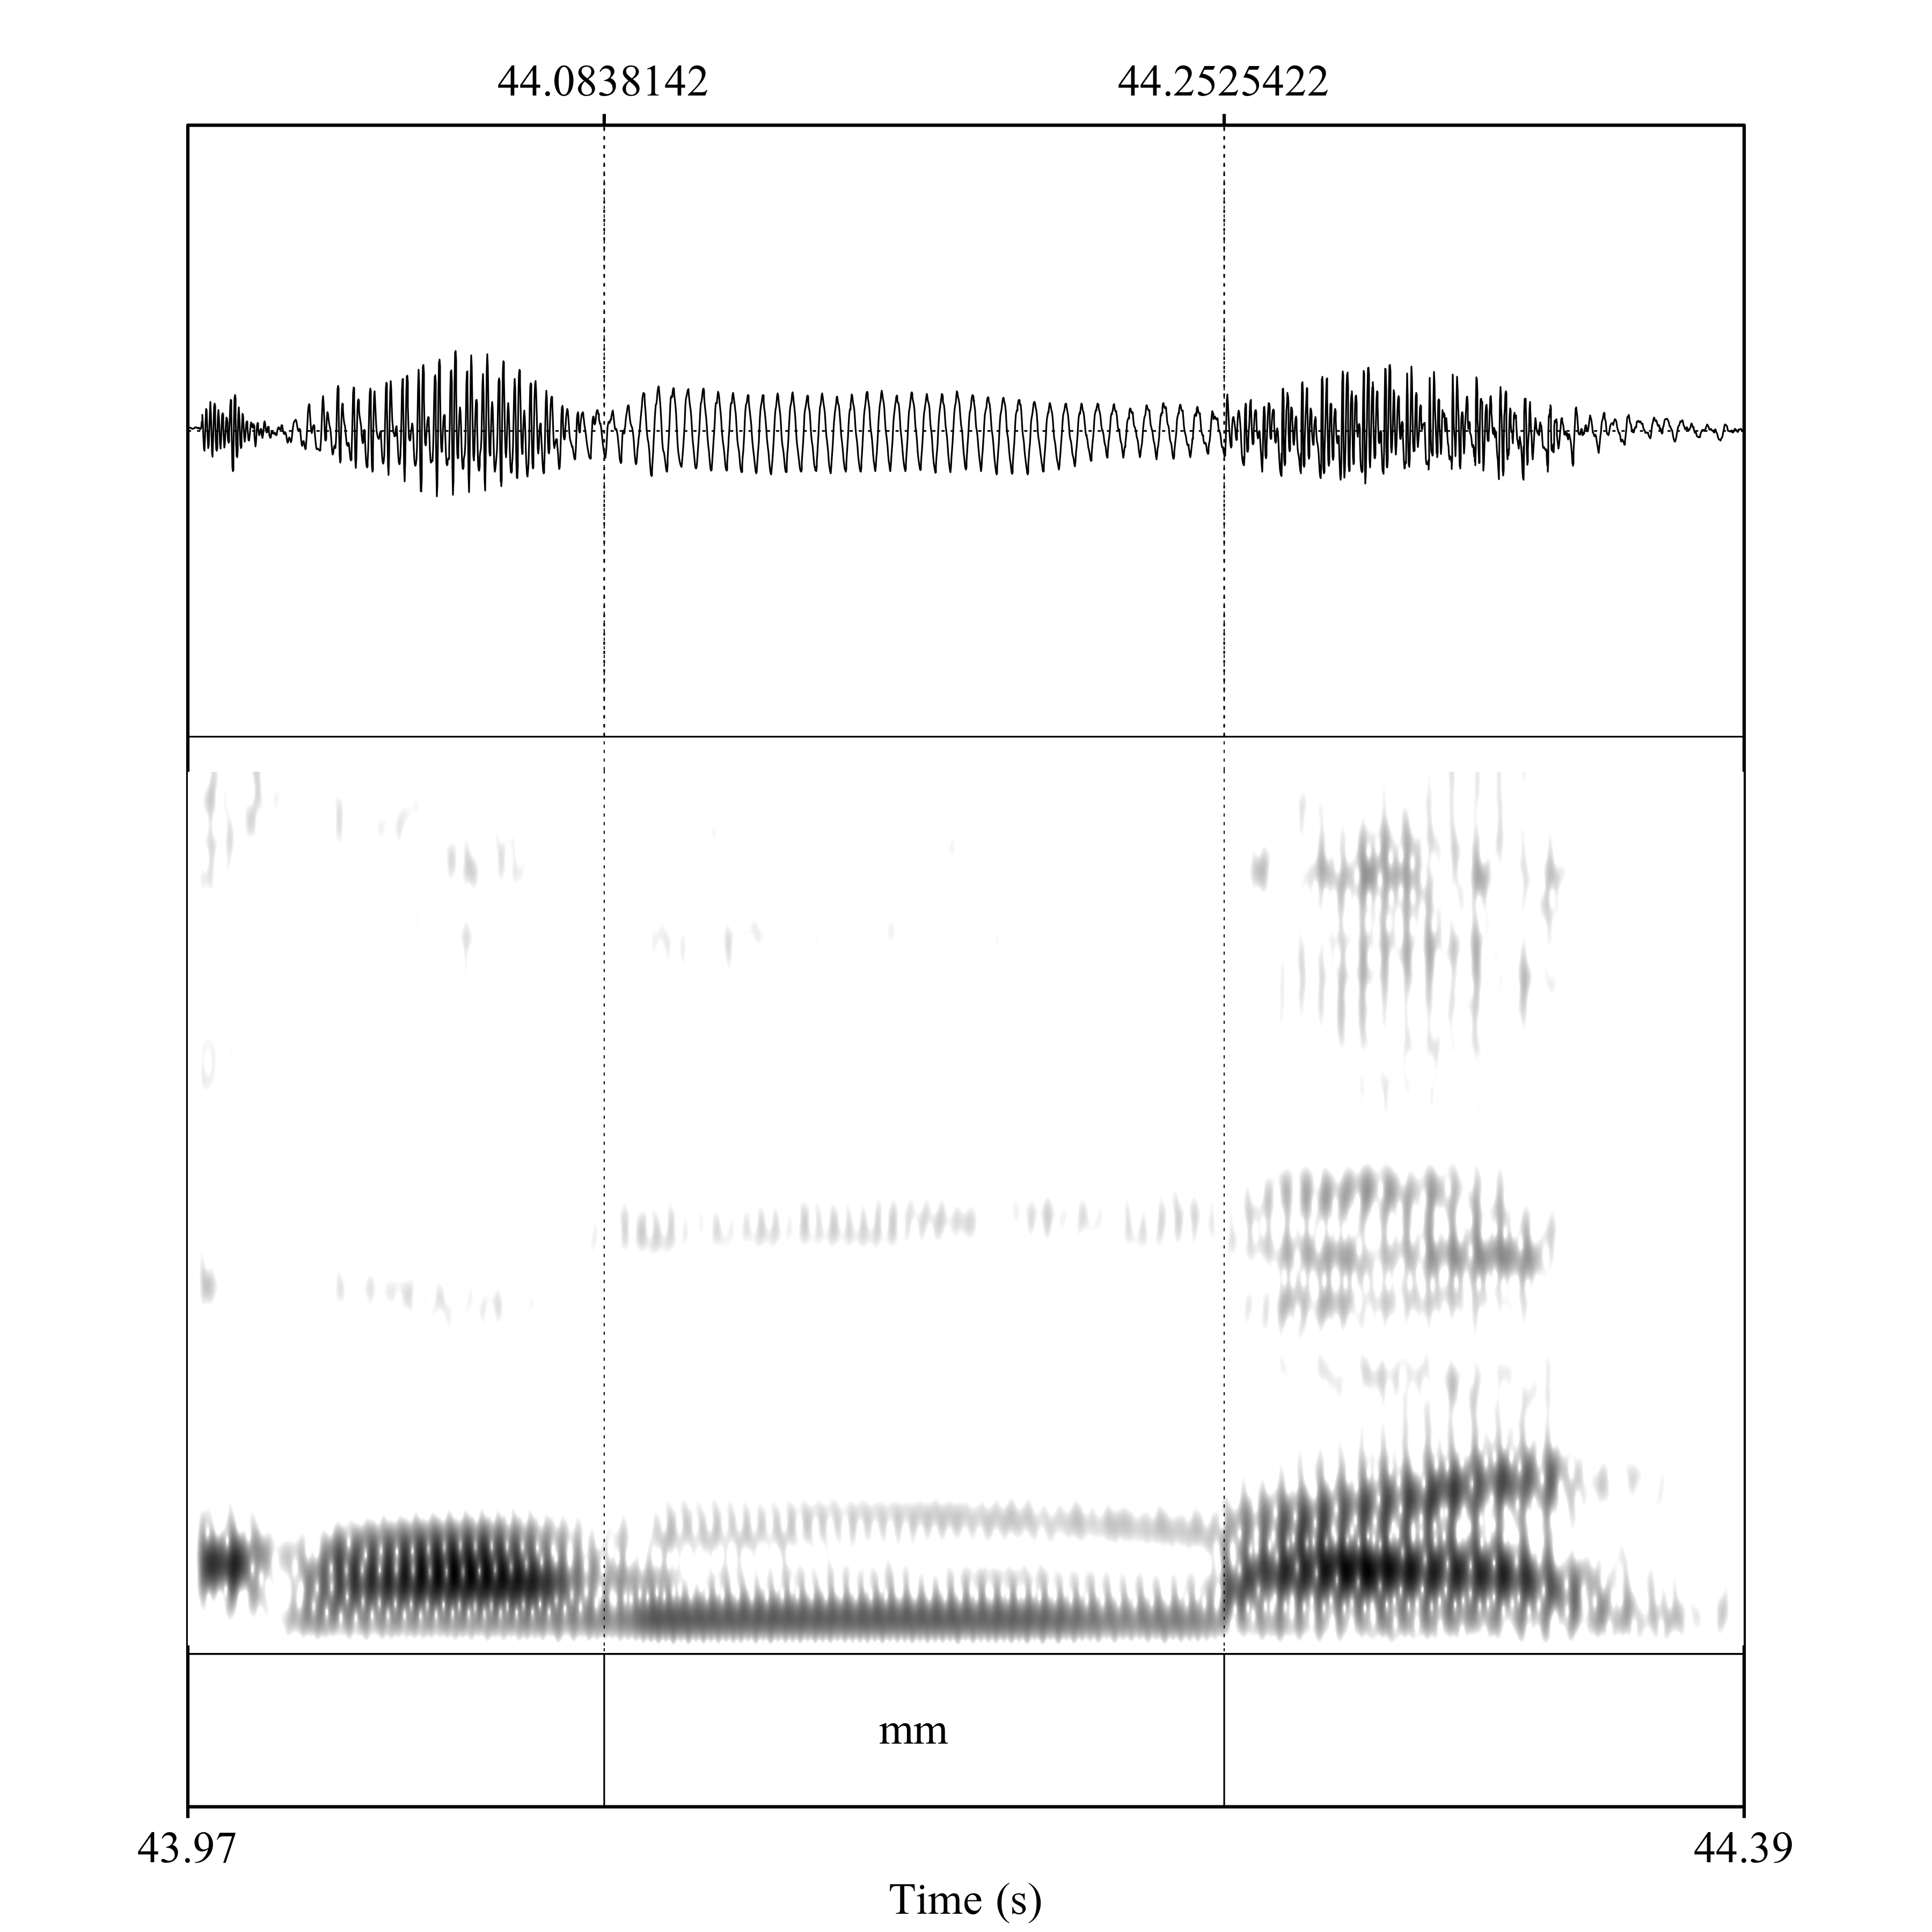
\includegraphics[width=0.7\linewidth]{kommoal.png}
\vspace{-0.4cm}\captionof{figure}{Measurement of {\ipa /mm/} in the word {\ipa /kommɔl/} 'to rest'}
\end{center}
}




%%%%%%


\headerbox{Results}{name=results,column=1,below=objectives,span=1}{
\begin{center}

        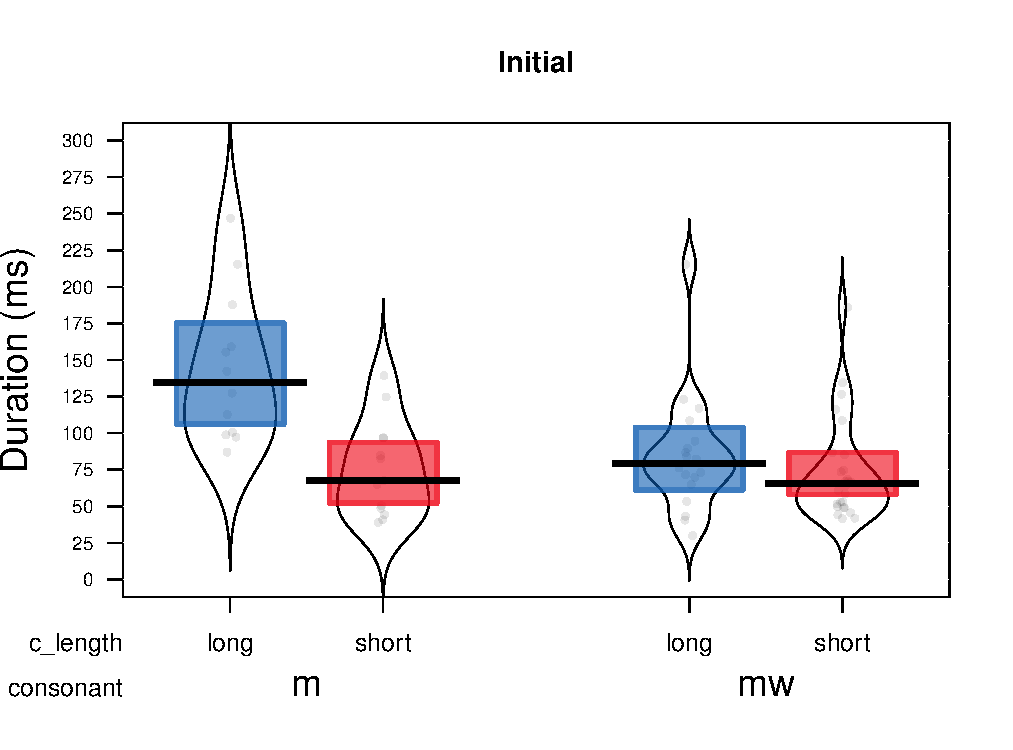
\includegraphics[width=0.9\textwidth]{initial.pdf}

        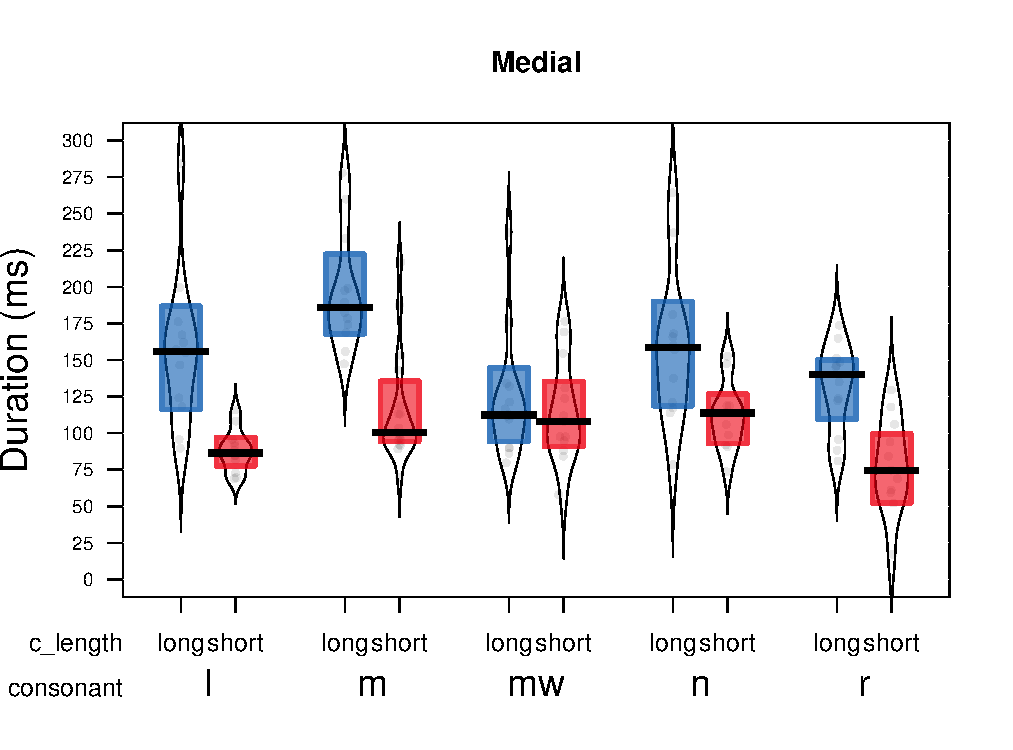
\includegraphics[width=0.9\textwidth]{medial.pdf}

        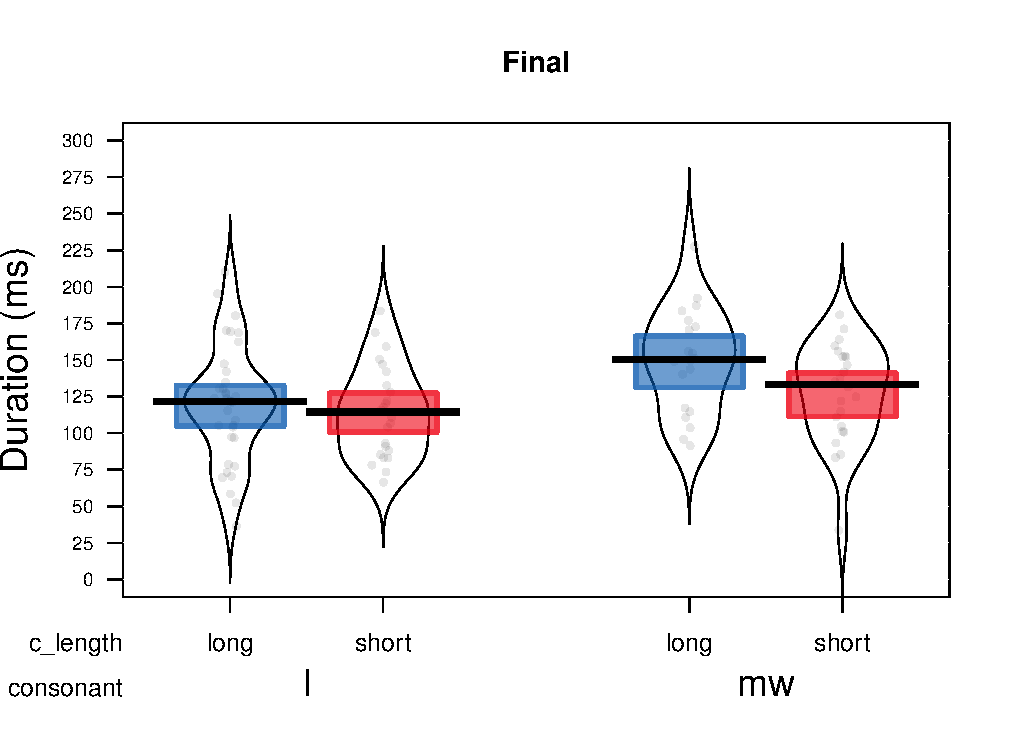
\includegraphics[width=0.9\textwidth]{final.pdf}


\vspace{-0.4cm}\captionof{figure}{Raw (data), Description, and Inference (RDI) plot of geminate vs. singleton segments by position in word}
\end{center}
}

\headerbox{BHLM Design}{name=bhlm,column=1,below=results,span=1}{

\begin{itemize}\compresslist
\item BHLM: duration \textasciitilde\ consonant length * consonant * frame + (1 + C length * consonant + frame | participant) +  (1 + C length * consonant + frame | word) [same for all three models]
\item Model Priors: \textbf{Intercept}: normal(0,20ms);\\ \textbf{Fixed effects}: normal(0,40ms); \textbf{Covariance}: regularization of 2 [same for all models]
\end{itemize}
}

\headerbox{References}{name=references,column=1,below=bhlm,span=1}{
\renewcommand{\section}[2]{\vskip 0.05em} % Get rid of the default "References" section title
%\nocite{*} % Insert publications even if they are not cited in the poster
\scriptsize{ % Reduce the font size in this block
\bibliographystyle{sp}
\bibliography{phon} % 
}
}

%%%%%%



\headerbox{Word Initial}{name=locus3,column=2,row=0}{

\begin{itemize}
\item No overlap of posterior 95\% credible interval\\ between geminates and singletons, which \\indicates a clear highly probable difference
\item {\ipa /m\textsuperscript{w}/} pairs did not have observed difference
\item Sentence frame had only small effect with\\ heavily overlapping credible intervals
\begin{itemize}\compresslist
\item Frame 3 (sentence medial) had the strongest difference, with the target segment being on average 40ms shorter than in other frames
\end{itemize}
\end{itemize}

\begin{center}
{\footnotesize
\begin{tabular}{l l l  l}
\toprule

&&\multicolumn{2}{c}{\textbf{CrI}}\\\cmidrule{3-4}
\textbf{Fixed effect} & \textbf{Mean (ms)} &  \textbf{2.5\%} & \textbf{97.5\%}\\
\midrule
Intercept & 158.69    &111.49&203.34\\
Length: short & --80.02  &    --150.63&--32.53\\
Frame 3 & --40.10 & --95.05 & 12.62\\

\bottomrule
\end{tabular}
}
\captionof{table}{Selected fixed effects of word initial BHLM}
\end{center}

\vspace{0.38em}
}

\headerbox{Word Medial}{name=moment2,column=2,below=locus3}{

\begin{itemize}\compresslist
\item Some overlap of posterior 95\% credible interval between geminates and singletons, which\\ indicates some probable similarity and also  some probability that singletons are shorter
\item {\ipa /m\textsuperscript{w}/} pairs did not have observed difference
\item Sentence frame had negligible effect with\\ heavily overlapping credible intervals

\end{itemize}

\begin{center}
{\footnotesize
\begin{tabular}{l l l  l}
\toprule

&&\multicolumn{2}{c}{\textbf{CrI}}\\\cmidrule{3-4}
\textbf{Fixed effect} & \textbf{Mean (ms)} &  \textbf{2.5\%} & \textbf{97.5\%}\\
\midrule
Intercept & 144.60    &78.88&209.83\\
Length: short & --45.12  &    --135.05&55.17\\
%Frame 3 & --40.10 & --95.05 & 12.62\\

\bottomrule
\end{tabular}
}
\captionof{table}{Selected fixed effects of word medial BHLM}
\end{center}

}


%%%%%
\headerbox{Word Final}{name=moment3,column=2,below=moment2}{

\begin{itemize}\compresslist
\item Strong overlap of posterior 95\% credible\\ interval between geminates and singletons:\\ improbable difference
\item {\ipa /m\textsuperscript{w}/} pairs did not have observed difference
\item Sentence frame had negligible effect with\\ heavily overlapping credible intervals

\end{itemize}

\begin{center}
{\footnotesize
\begin{tabular}{l l l  l}
\toprule

&&\multicolumn{2}{c}{\textbf{CrI}}\\\cmidrule{3-4}
\textbf{Fixed effect} & \textbf{Mean (ms)} &  \textbf{2.5\%} & \textbf{97.5\%}\\
\midrule
Intercept & 118.42    &91.73&145.80\\
Length: short & --6.61  &    --42.85&30.00\\
%Frame 3 & --40.10 & --95.05 & 12.62\\

\bottomrule
\end{tabular}
}
\captionof{table}{Selected fixed effects of word final BHLM}
\end{center}

}



%----------------------------------------------------------------------------------------
%	CONCLUSION
%----------------------------------------------------------------------------------------

\headerbox{Conclusions}{name=conclusion,column=2,below=moment3}{

\begin{itemize}\compresslist

\item We observed geminate/singleton contrasts word \textbf{initially} and \textbf{medially}, but  \textbf{not} finally,\\ contrary to \citet{Rehg:1981}
\item {\ipa /m\textsuperscript{w}/} did not have any observed \\geminate/singleton contrasts



\end{itemize}


}


%----------------------------------------------------------------------------------------
%	CONTACT INFORMATION
%----------------------------------------------------------------------------------------

\headerbox{Contact Information}{name=contact,column=2,below=conclusion}{ % This block is as tall as the references block
\scriptsize{
\begin{description}\compresslist
\item[Web] http://rentz.weebly.com
\item[Email] rentzb@hawaii.edu, vanderso@hawaii.edu
\item[Data \& Code] github.com/rentzb/pape
\end{description}



}}

\headerbox{Acknowledgments}{name=ackno,column=2,row=3,below=contact}{
\begin{singlespace}\scriptsize{We thank Amy Schafer, William O’Grady, Ken Rehg, Robert Andreas, and Damian Sohl for their help  with this project. Most of all we thank Linda Kihleng-Albert, Maurina Ludwig, Dusty Santos, Joshua Fredrick, and Robinson Fredrick for sharing their knowledge and allowing us to write about their language. Kalahngan en kupwuromwail!
}\end{singlespace}}


\end{poster}

\end{document}